\section{Proposed ChatBot}
%
\subsection{DataModel}
It seems obvious that browsing our 2,249,053 lines-long corpus for each query wasn't such a great idea, that's why we stored the data in a re-usable DBMS.
\subsubsection{Chosen technology}
We considered 2 options : a traditional DBMS such as MySQL or a graph-oriented DBMS. We finally chose to use a graph model for several reasons :
\begin{itemize}
\item For a corpus such as ours, with a lot of n-1..n relations, a graph allows the user to build queries who look like \say{paths}. It is both more efficient (no table join, less computation time) and more natural for the user.
\item Graph-base DBMS doesn't require a rigid schema, which means that we can create new kind of entities and relationships \say{on the go}.
\item It supports indexes and unique constraints
\item Most of the graph-based systems implements useful algorithms such as the shortest path between two nodes.
\end{itemize}
Regarding the technology, Neo4j\footnote{http://neo4j.com/} was chosen in regards of those facts :
\begin{itemize}
\item One of us (Mael) was already working with it for his MasterArbeit and was familiar with the language used to build Neo4j queries (Cypher).
\item Neo4j is cross-platform
\item The community is strong, there're even french groups
\item The technology is mature, 15 years old and currently running version 2.2
\item It provides a nice browser interface
\end{itemize}

\subsubsection{Structure}
Here, we will describe the actual structure of the corpus-graph. Remember that it isn't rigid so it might vary over the project's progress.\\
Other nodes and relationships exist in our database but are used for other purposes such as the history of the conversation or some probabilities (see section \ref{sssec:v_stype}).\\
Basically we can say that in our case, one vertex equals one XML tag. Instead of listing all the vertexes and the edges, we provide here an example based on a dialogue from the movie\footnote{12 Monkeys on IMDB : http://www.imdb.com/title/tt0114746/} \say{12 Monkeys}.
\lstinputlisting[language=XML,caption=XML extract,label={code:extr}]{./prim/graphExample.xml}
\begin{figure}[!h]
\begin{center}
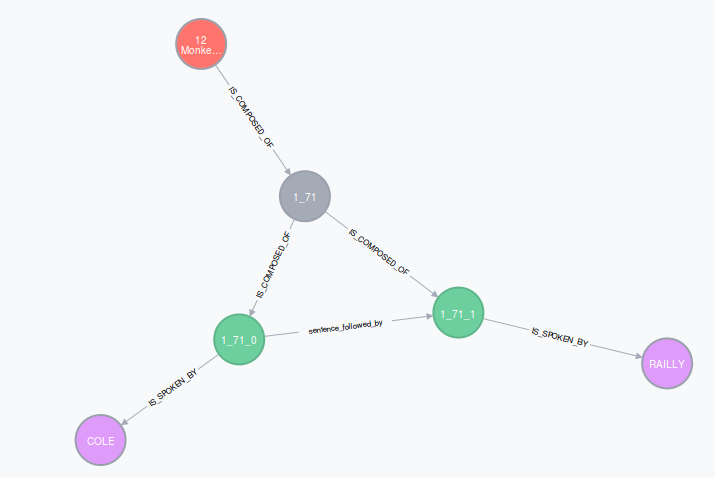
\includegraphics[width=0.8\textwidth]{./img/graph171.png}
\end{center}
\caption{Neo4j modelisation}
\label{fig:neoExtr}
\end{figure}
With the above example we see that, just like in the XML (Code \ref{code:extr}), a \textbf{Movie} (pink) \textit{IS\_COMPOSED\_OF} \textbf{Dialogues} (gray, only one displayed here) which \textit{IS\_COMPOSED\_OF} several \textbf{Sentences} (green). Each sentence \textit{IS\_SPOKEN\_BY} a \textbf{Character} (purple).\\
We store the full sentence as an attribute of the Sentence node. The labels of the dialogues and sentences are an aggregation of the id fields of their parents :
\begin{center}Sentence\_Node\_id = idMovie\_idDialogue\_idSentence \end{center}
Now that we have represented the corpus as a graph, we can start to work with the NLP technology. Each sentence is processed and we use the nltk library to tokenize and tag all sentences in our corpus. The purpose of the processing is to identify for each sentence its type and the most relevant tokens. These informations will be then used by anna to answer with the sentence wich is the most relevant given previous sentences.\\
We identify four categories of sentence : interrogative, exclamative, affirmative and greeting. Moreover a sentence can be either negative or positive. To determine if a sentence is interrogative or exclamative we check the presence of a question mark (?) or a exclamation point (!) at the end of the sentence. If no such marks is found we assume that the sentence is affirmative. To determine if a sentence is negative we check if the sentence contain a \say{n't} token. Finally to detect a greeting we check if the sentence contain keywords such as \say{Hi}, \say{Hello}, \say{Good Morning}\dots\\
Regarding the tokens we assume tokens tagged as noun and verb are the most relevant to understand the meaning of the sentence and thus we only keep these and eliminate others.\\
The figure \ref{fig:sent} illustrate the informations stored in the database.

\begin{figure}[!h]
\begin{center}
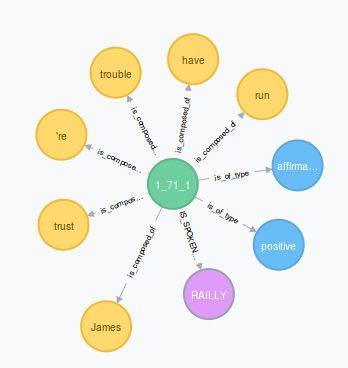
\includegraphics[width=0.5\textwidth]{./img/graph1711.png}
\end{center}
\caption{Sentence details}
\label{fig:sent}
\end{figure}

%
\subsection{User Interface}
\subsubsection{Chosen technology}
\label{subs:Technology}

\paragraph{State of the Art}
\label{par:SotA}
Obviously, this is a Python project, because the point of the course is to discover NLP and Text-mining by using NLTK.
So, we decided to naturally go and try our way in Python to get an interface for our chat-bot.
In the litterature, there are two main approaches for doing that :
\begin{itemize}
    \item Interfacing our bot on an IRC server, and using an IRC client as a User Interface.
    \item Developing our own interface.
\end{itemize}
As we wanted the user to be able to rate our bot's answers, the first solution was never really an option.
An IRC (or so) client's interface doesn't give us room for non-textual interaction, and it is something which was important for us.
The second solution, developing our own interface, is quite easy in Python, as long as you have more than just notions in web development.
We explored two Python frameworks, \textit{Django} and \textit{Flask}.
\textit{Django} is obviously way too dense and heavy for our needs, so we tried our best with Flask.
Considering that the user interface is not a very important component of our application, we decided that Flask was also a waste of time for us, and that we should do what we could already do.

\paragraph{Shiny}
\label{par:Shiny}
Therefore we decided to propose a R user interface.
R is, like Python, an open-source interpreted language, but it is specialized in Data Mining.
Its main IDE, RStudio, proposes a package for building easily interactive web interfaces.

\paragraph{Interfacing R with Python}
\label{par:rPython}
The point of the project still being to develop a chat-bot based on NLP and text-mining (in Python, using NLTK), we figured out a way of connecting both, and built APIs to do it easily.
Our app is called through R interpreter, which launches the User Interface. Then, the R server calls for the answering API, which eventually calls Python answering engine.

\newpage
\subsubsection{Result}
\label{subs:Result}

\begin{figure}[!h]
\begin{center}
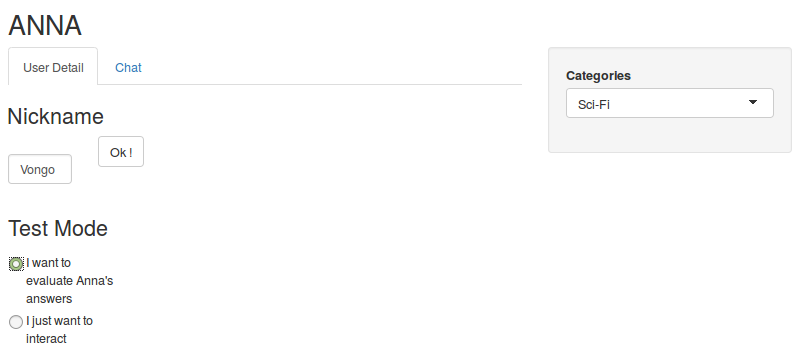
\includegraphics[width=0.70\textwidth]{./img/AnnaLoginUI.png}
\end{center}
\caption{LogIn Interface, where you can also decide whether you want to evaluate Anna's answers.}
\label{fig:AnnaLoginUI}
\end{figure}

\begin{figure}[!h]
\begin{center}
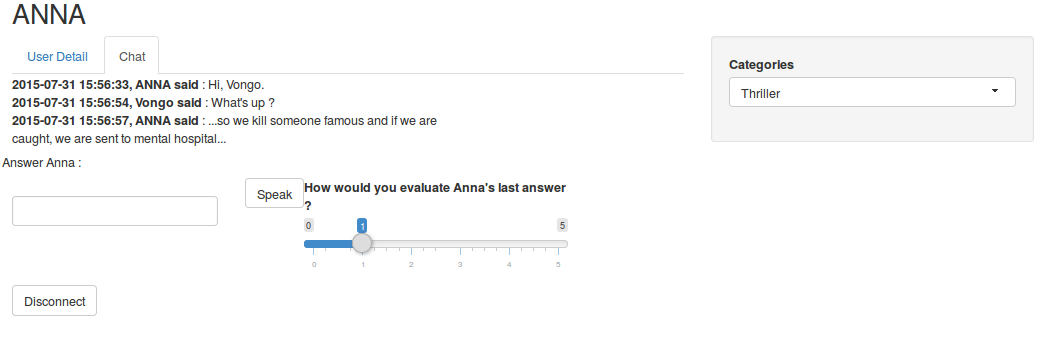
\includegraphics[width=0.80\textwidth]{./img/AnnaChatUI.png}
\end{center}
\caption{Chat Interface : a simple chat session.}
\label{fig:AnnaChatUI}
\end{figure}

\subsection{Architecture}
\label{sub:Architecture}

If we take a look at Figure~\ref{fig:Archi}, we can see that the responsibilities given to R and Python are not the same.
R is in charge of :
\begin{itemize}
    \item The User Interface, both for the cosmetic and the behavioural part.
    These components will also be responsible for calling Python API through an elegant R API, thanks to the library \textit{rPython\footnote{$rpython.r-forge.r-project.org/$}}.
    \item Building the statistics on the new data we get on the web.
    For that matter, we use built-in R, as well as \textit{ggplot2\footnote{$ggplot2.org/$}} library.
    For cooccurrences graphs, we build cooccurrence matrices, that we read and display with Gephi\footnote{$gephi.github.io/$}.
    \item Taking into account the user's evaluations\footnote{In a later version.}.
\end{itemize}

On the other hand, Python is in charge of :
\begin{itemize}
    \item Retrieving information about the movies through OMDb API\footnote{$www.omdbapi.com/$}.
    \item Parsing the XML dataset\footnote{$docs.python.org/2/library/xml.html$} to build the neo4j graphbase\footnote{$py2neo.org/$}.
    \item Finding the best answer for a given conversation (Confer \ref{sub:Answering}).
\end{itemize}

\begin{figure}[!h]
\begin{center}
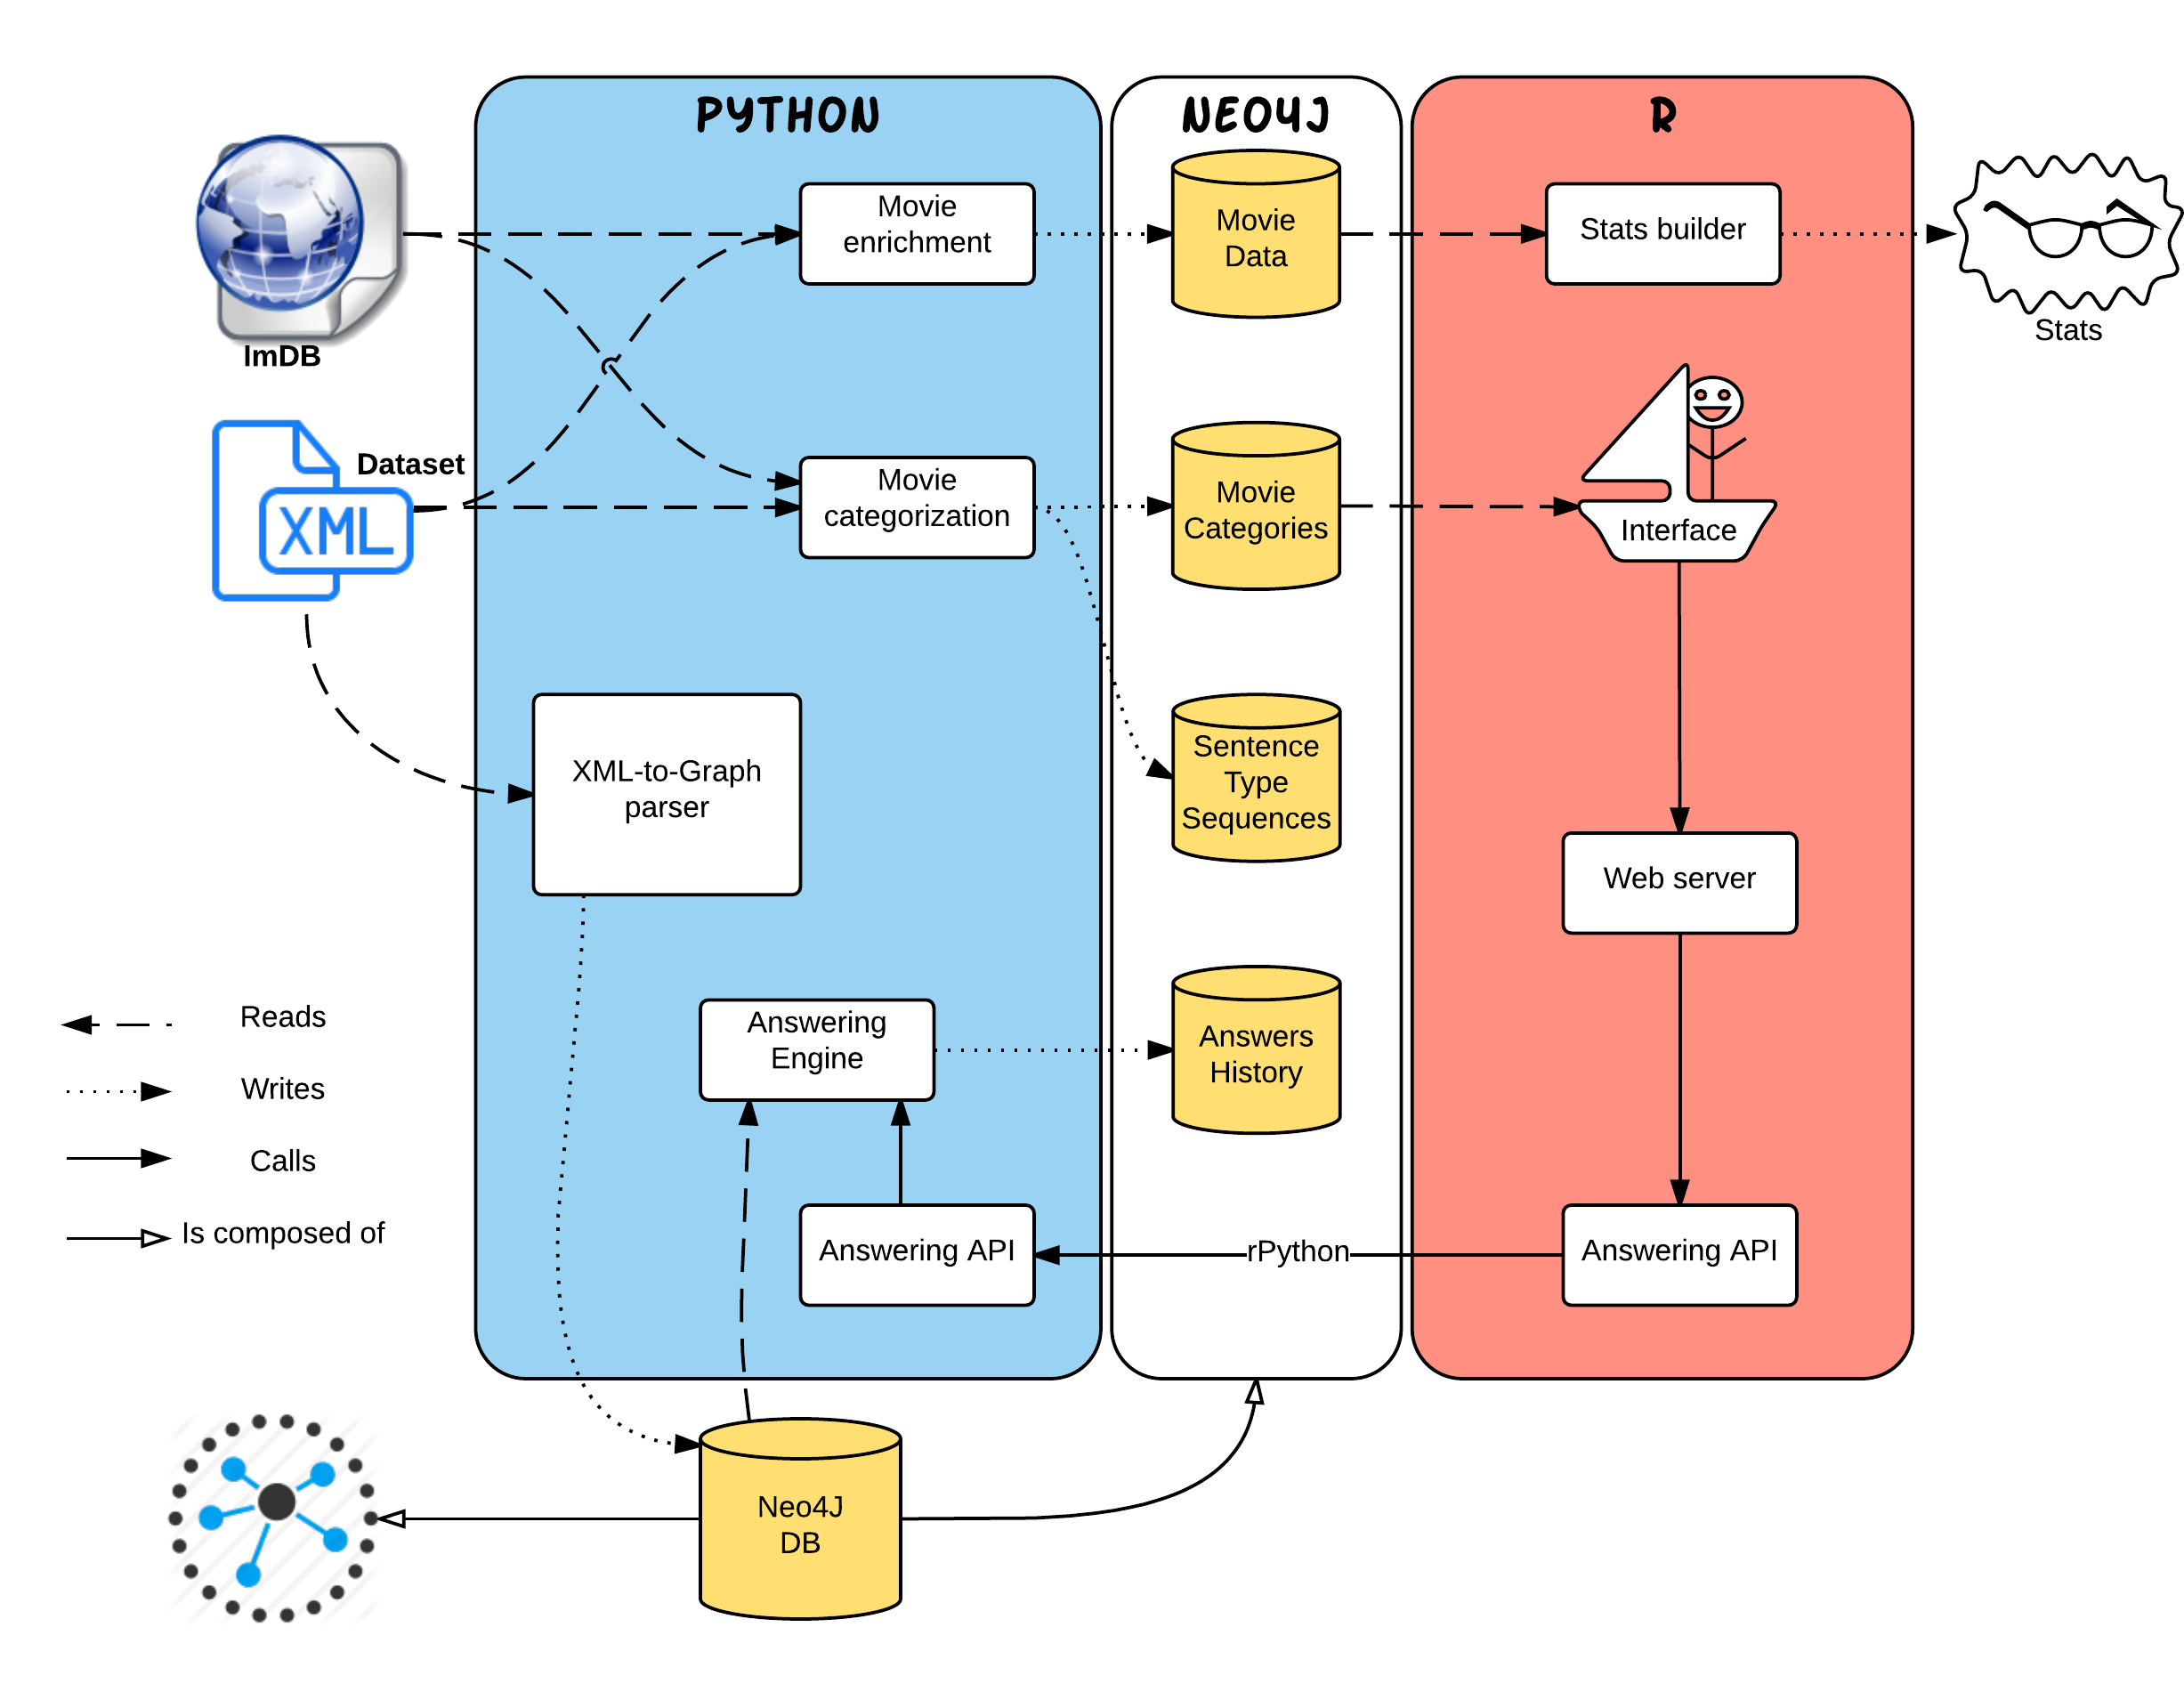
\includegraphics[width=1.1\textwidth]{./img/Archi.png}
\end{center}
\caption{Anna's Architecture.}
\label{fig:Archi}
\end{figure}

%
\subsection{Anna's answers}
\label{sub:Answering}

\subsubsection{Version 1 : Random answers}
\label{sssec:v_rand}
There is not much to say about this first release. Like in all projects, we implemented a basic and stupid version to make sure that all communications processes (between R and Python for instance) are correctly working and that our queries to the graph are successful.\\
Anna's answer is selecting with the help of 3 random functions. First, we randomize the amount of movies in the graph : idMovie.\\
Then, the average of dialogues per movie beeing 175.60, we get a random dialogue by randomizing between 0 and 100 : idDialogue.\\
The sentence's id is also random, between 0 and the number of outgoing \textit{IS\_COMPOSED\_OF} relationships from the above dialogue : idSentence.\\
And the winner is : idMovie\_idDialogue\_idSentence !\\
This results on conversations which make no sense at all, see Figure \ref{fig:convRandom} for an example.\\
\begin{figure}[!h]
\begin{center}
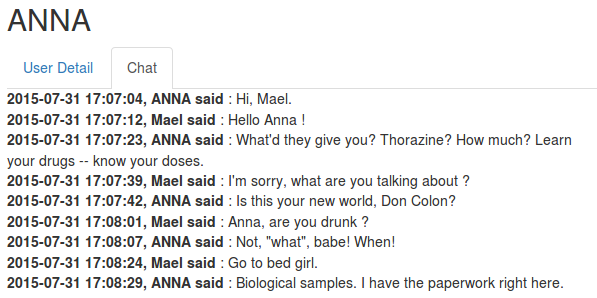
\includegraphics[width=0.80\textwidth]{./img/convRandom.png}
\end{center}
\caption{Random conversation from V1}
\label{fig:convRandom}
\end{figure}
\subsubsection{Version 2 : Determined SentenceType}
\label{sssec:v_stype}
\begin{figure}[!h]
\begin{center}
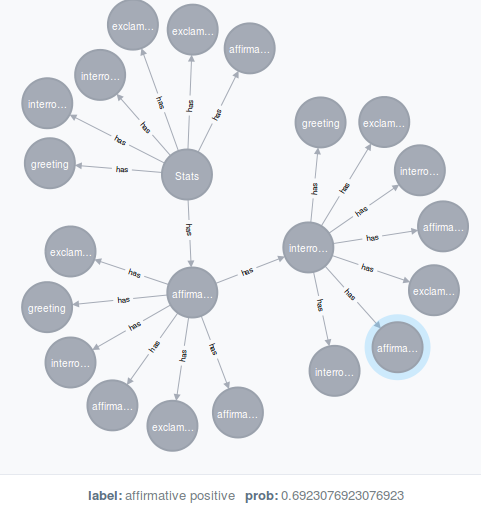
\includegraphics[width=0.6\textwidth]{./img/stats.png}
\end{center}
\caption{Probabilities tree}
\label{fig:stats}
\end{figure}
For the second release of the project we use likelihood to determine the best type of sentence to answer.\\
The first step is to run through all dialogues in our corpus and compute for each sequence of sentence's type the probabilities of the types of the following sentence. To do so we first start by computing probabilities with a sequence of length 1 meaning for each possible sentence's types (affirmative positive, affirmative negative, interrogative positive...) we look at the types of the following sentences and compute probability of occurrence for each type. Then we repeat the process for a sequence of length 2 (affirmative positive - affirmative negative, affirmative positive - interrogative positive...) then sequence of length 3 and so on.\\
The results are stored as a graph where each node represent a sentence's type associated with its probability of occurrence given previous sentence's type represented by its ancestors in the tree.\\
Figure \ref{fig:stats} displays a 3-depth graph of probabilities in which we can see that, after the sequence \say{affirmative positive -- interrogative positive}, the probability of the SentenceType \say{affirmative positive} is of 69\%.\\
Then when Anna is speaking with an user we use these statistics to answer a sentence whose type is the most likely to occur given the types of the previous sentences in the dialogue. It results on conversations which are correctly structured. See figure \ref{fig:convST} for a creepy example.
\begin{figure}[!h]
\begin{center}
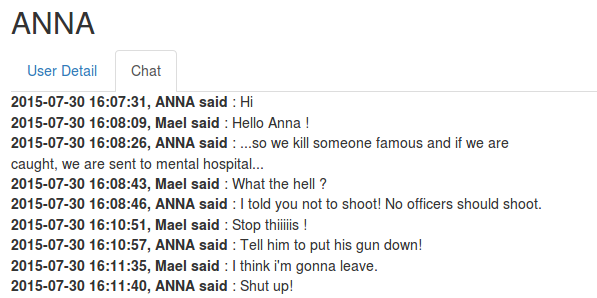
\includegraphics[width=0.80\textwidth]{./img/convST.png}
\end{center}
\caption{Conversation from V2}
\label{fig:convST}
\end{figure}
\subsubsection{Version 3 : Determined movie genre}
\label{sssec:v_genre}
